\documentclass[11pt,letterpaper]{article}
\pdfinfoomitdate=1
\pdftrailerid{}
\pdfsuppressptexinfo=-1
\usepackage[T1]{fontenc}
\usepackage[utf8]{inputenc}
\usepackage{lmodern,microtype}
\usepackage[margin=0.85in,top=0.85in,bottom=0.85in,headheight=14pt]{geometry}
\usepackage{amsmath,amssymb,graphicx,booktabs,array,longtable,xcolor}
\usepackage{tikz}
\usetikzlibrary{arrows.meta,positioning,fit,backgrounds}
\usepackage[font=small,labelfont=bf,labelsep=period]{caption}
\usepackage[numbers,sort&compress]{natbib}
\usepackage{titlesec}
\usepackage{enumitem}
\usepackage{fancyhdr}
\usepackage{placeins}
\definecolor{ink}{HTML}{183E53}
\definecolor{accent}{HTML}{17668B}
\definecolor{warm}{HTML}{AD5528}
\definecolor{muted}{HTML}{555F65}
\definecolor{pale}{HTML}{F0F5F7}
\usepackage[colorlinks=true,linkcolor=accent,citecolor=accent,urlcolor=accent,
pdftitle={Scalable Meta-Learning from Hindsight},pdfauthor={Angel Raychev},
pdfsubject={Learning policy targets from completed experience},
pdfcreator={LaTeX}]{hyperref}
\urlstyle{same}
\titleformat{\section}{\large\bfseries\color{ink}}{\thesection}{0.6em}{}
\titleformat{\subsection}{\normalsize\bfseries}{\thesubsection}{0.6em}{}
\titlespacing*{\section}{0pt}{2.2ex plus .8ex minus .2ex}{1ex plus .2ex}
\titlespacing*{\subsection}{0pt}{1.7ex plus .5ex minus .2ex}{.7ex plus .2ex}
\setlength{\parindent}{0pt}
\setlength{\parskip}{5.4pt plus 1pt minus .5pt}
\setlength{\emergencystretch}{2em}
\setlength{\tabcolsep}{5pt}
\renewcommand{\arraystretch}{1.17}
\setlist{nosep,leftmargin=1.5em,topsep=5pt}
\renewcommand{\topfraction}{.92}
\renewcommand{\bottomfraction}{.85}
\renewcommand{\textfraction}{.08}
\renewcommand{\floatpagefraction}{.75}
\clubpenalty=10000
\widowpenalty=10000
\displaywidowpenalty=10000
\pagestyle{fancy}
\fancyhf{}
\fancyhead[L]{\small\color{muted}Scalable Meta-Learning from Hindsight}
\fancyhead[R]{\small\color{muted}Angel Raychev}
\fancyfoot[L]{\small\color{muted}Technical report \textperiodcentered{} October 2026}
\fancyfoot[R]{\small\color{muted}\thepage}
\renewcommand{\headrulewidth}{0pt}
\newcommand{\KL}{D_{\mathrm{KL}}}
\newcommand{\sg}{\operatorname{sg}}
\newcommand{\score}{J}
\newcommand{\code}[1]{\texttt{#1}}
\newcolumntype{L}[1]{>{\raggedright\arraybackslash}p{#1}}
\newcolumntype{R}[1]{>{\raggedleft\arraybackslash}p{#1}}
% Presentation revision only. The scientific source and original macros remain.
\usepackage{angel-publication}
\PublicationRunningTitle{Scalable Meta-Learning from Hindsight}
\PublicationRunningAuthor{Angel Raychev}
\PublicationStatus{Presentation revision - 24 October 2026}
\begin{document}
\thispagestyle{plain}
\begin{center}
{\PublicationTitleFont Scalable Meta-Learning\\[3pt]from Hindsight\par}
\vspace{9pt}
{\large Learning policy targets from completed experience\par}
\vspace{10pt}
{\normalsize Angel Raychev\par}
\vspace{5pt}
{\small\color{muted}24 October 2026\par}
\vspace{6pt}
\PublicationLinks{https://angelraychev.com/scalable-meta-learning-from-hindsight/}{https://github.com/RaychevAngel/learning-from-hindsight}
\end{center}
\vspace{2pt}
\begin{abstract}
\noindent
A completed experience reveals information that was unavailable while an agent acted. We investigate how to turn that information into a parameter update that helps on different tasks. A source-restricted proposer supplies candidate privileged-information contexts; matched student updates measure their learning value; and a future-aware teacher learns to assign the selected policy distributions directly from raw completed experience. This teacher predicts full-vocabulary targets rather than generating a lesson or replacement answer. We implement the distribution, update and black-box proposer-training interfaces, and study their components with Qwen3.5-4B on algorithmic array transformations. On fresh source experiences, hindsight-teacher fitting reduces mean forward KL to selected references from 0.2791 to 0.0583. Contextual lessons are useful, but this fidelity gain does not establish reliable downstream benefit: causal query scores are 30/64 for the fitted-teacher update, 27/64 without updating and 28/64 for an unfitted teacher, with source-cluster intervals spanning zero. An independent distribution audit finds that 98.54\% of summed initial source KL lies in verbal rule text, while corrective targets at erroneous array entries remain weak or unevenly fitted. These results separate contextual utility, distribution assignment and durable student improvement, and motivate optimizing teaching by the learning it actually causes.
\end{abstract}

\section{Learning from experience rather than explaining it}

An agent finishes a task with evidence it did not possess when making its earlier decisions: a failed test, a tool result, an unexpected outcome, or a correction that finally worked. A useful learning system should turn this experience into better future behavior. Producing a convincing retrospective explanation is not the same achievement.

The proposal investigated here is to \emph{learn the teaching procedure}. During an expensive outer loop, a proposer reads a completed source experience and suggests privileged-information contexts, abbreviated PI. Each context conditions a snapshot of the model and changes the distributions it assigns to the source's original action prefixes. Matched student clones learn from these distributions. Their subsequent performance on different tasks, with the PI absent, measures the candidate's learning value.

The selected distributions then supervise a hindsight teacher. Given only the raw completed experience, this model predicts the policies induced by useful teaching interventions. It need not reconstruct the lesson, generate a corrected response or sample a new trajectory. The intended amortized update is a scoring pass over existing experience followed by causal distillation.

This design makes three questions explicit:
\begin{enumerate}
\item Does the source-derived information help a model while it is in context?
\item Can a raw-experience teacher learn to assign the selected distributions?
\item Do updates from those distributions improve a causal student on different tasks?
\end{enumerate}
The empirical study shows why these cannot be collapsed into one success metric. It contains positive component-level transfer, fresh-source distribution generalization and detailed numerical diagnostics, but does not establish reliable improvement from the complete learned procedure.

The implemented contribution comprises source-restricted proposal and selection, matched student/optimizer resets, detached full-vocabulary targets, aligned scoring of original action tokens, future-aware teacher fitting, actual-update-reward proposer optimization, and independent evidence reconstruction. The experiments evaluate these components rather than a production continual-learning system.

\section{The learning procedure}
\label{sec:method}

\begin{figure}[t]
\centering
\begin{publicationdiagram}
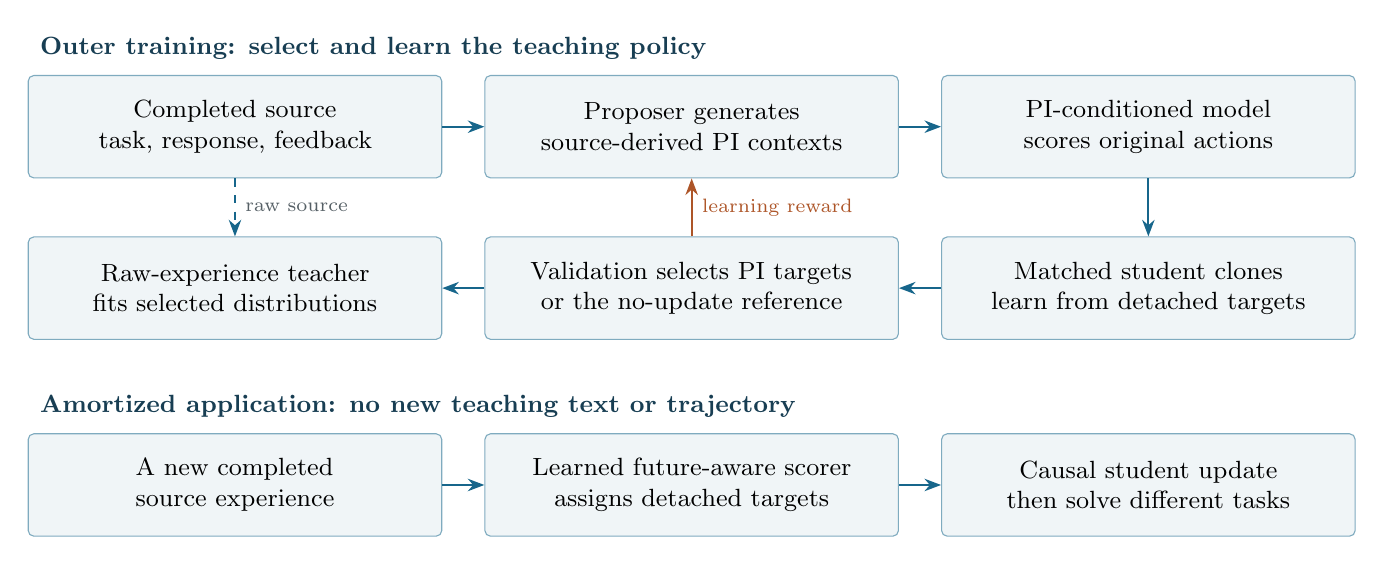
\begin{tikzpicture}[
  box/.style={draw=accent!55,fill=pale,rounded corners=2pt,align=center,
    text width=4.9cm,minimum height=13mm,inner sep=5pt,font=\small},
  arrow/.style={-{Stealth[length=2.1mm]},thick,draw=accent},
  note/.style={font=\small\bfseries,text=ink,anchor=west}
]
\node[note] at (0,1.0) {Outer training: select and learn the teaching policy};
\node[box] (s) at (2.6,0) {Completed source\\task, response, feedback};
\node[box] (p) at (8.4,0) {Proposer generates\\source-derived PI contexts};
\node[box] (q) at (14.2,0) {PI-conditioned model\\scores original actions};
\node[box] (u) at (14.2,-2.05) {Matched student clones\\learn from detached targets};
\node[box] (v) at (8.4,-2.05) {Validation selects PI targets\\or the no-update reference};
\node[box] (h) at (2.6,-2.05) {Raw-experience teacher\\fits selected distributions};
\draw[arrow] (s)--(p); \draw[arrow] (p)--(q); \draw[arrow] (q)--(u);
\draw[arrow] (u)--(v); \draw[arrow] (v)--(h);
\draw[arrow,draw=warm] (v.north)--node[right,font=\scriptsize,text=warm]{learning reward}(p.south);
\draw[arrow,dashed] (s)--node[right,font=\scriptsize,text=muted]{raw source}(h);
\node[note] at (0,-3.55) {Amortized application: no new teaching text or trajectory};
\node[box] (s2) at (2.6,-4.55) {A new completed\\source experience};
\node[box] (h2) at (8.4,-4.55) {Learned future-aware scorer\\assigns detached targets};
\node[box] (u2) at (14.2,-4.55) {Causal student update\\then solve different tasks};
\draw[arrow] (s2)--(h2); \draw[arrow] (h2)--(u2);
\end{tikzpicture}
\end{publicationdiagram}
\caption{Learning teaching value and amortizing its policy effect. Validation measures the student with PI absent. Queries compare the fixed procedure. The application path eliminates additional \emph{target-generation sampling}, not scoring, optimization or the original source rollout.}
\label{fig:loop}
\end{figure}


\subsection{Source experience and information boundaries}

Let $\tau=(x,a_{1:T},f)$ be a completed source experience. The public task is $x$, the original response $a_{1:T}$ was generated by causal actor $p_{\theta_0}$, and $f$ is observed feedback. For interactive settings, observations would also be part of the history; the present tasks use a single response and binary correctness feedback. The actor's response positions are the supervised actions. Feedback can inform teaching, but is not an action label.

Related validation tasks $V$ score candidate-induced updates. Query tasks $Q$ compare the resulting students after the procedure is fixed within a comparison. A truly untouched final test is a separate role. All reported query sets are development evidence, repeatedly inspected during research.

A proposer $g_\psi(z\mid\tau)$ receives one source experience as its instance-specific evidence. It does not receive validation/query tasks, their answers, family identifiers or other source episodes. The main component comparisons use one unedited lesson per source from a fixed external proposer session; they do not establish that the proposer has learned. This source-only restriction was enforced through the supplied instructions and inputs, not independently certified as a sandbox security boundary.

\subsection{Turn a candidate lesson into a distribution}

A candidate PI context $z$ conditions a frozen causal snapshot to form
\begin{equation}
q_{z,t}(\cdot)=p_{\theta_0}(\cdot\mid z,x,a_{<t}).
\label{eq:pi}
\end{equation}
The model does not generate a replacement answer. It scores every original action prefix. The response's original token IDs are retained when PI changes the prompt length, and each action uses its predecessor-position logits. Teacher and student therefore score the same actions despite different prompt offsets.

For a bounded $K$-step update $U_K$, the student minimizes
\begin{equation}
\mathcal L_S(\theta;q_z,\tau)
=\frac1T\sum_{t=1}^{T}
\KL\!\left(\sg[q_{z,t}]\;\middle\|\;
p_\theta(\cdot\mid x,a_{<t})\right),
\qquad
\theta_z=U_K(\theta_0;q_z,\tau).
\label{eq:student}
\end{equation}
The target is detached by $\sg$. The main comparisons use temperature one and full-vocabulary forward KL, not a top-$k$ approximation or a sampled-token policy-gradient estimate. Every candidate begins at the same student parameters with a fresh optimizer state.

These rollouts are on-policy for their declared initial actor snapshot. Multiple update steps reuse frozen historical prefixes rather than resampling after each step. If a target favors correcting an earlier token, later targets still condition on the historical prefix. This is a finite replay update, not continuously refreshed on-policy sampling.

\subsection{Measure teaching by post-update performance}

The authoritative candidate reward is
\begin{equation}
R_{\mathrm{update}}(z;\tau,V)
=\score_V(p_{\theta_z})-\score_V(p_{\theta_0}),
\label{eq:reward}
\end{equation}
with both policies evaluated causally and without PI. Select the best candidate found under the declared budget, allowing no update and preferring it on ties. The neutral reference is then the original causal source distribution. This is a bounded search result, not a globally optimal intervention.

The proposer can learn from this black-box reward using policy-gradient or preference procedures. There is no requirement to differentiate through $U_K$. Avoiding second-order differentiation nevertheless leaves the costs of proposal generation, target scoring, matched updates and validation.

A cheaper surrogate evaluates the PI directly in validation-task prompts:
\begin{equation}
R_{\mathrm{context}}(z;\tau,V)
=\score_V\bigl(p_{\theta_0}(\cdot\mid z)\bigr)-\score_V(p_{\theta_0}).
\label{eq:context}
\end{equation}
The source-derived lesson is reused, not rewritten after seeing each validation task. This measures contextual utility, not parameter transfer. To use it as a ranking surrogate requires paired candidate-level validation; the direct-context condition comparisons below do not establish that correlation.

\subsection{Amortize the policy assignment}

Let $q_t^*(\tau)$ be the selected PI or neutral reference at each original action position. A hindsight teacher $h_\phi$ learns
\begin{equation}
\mathcal L_H(\phi)
=\mathbb E_\tau\!\left[
\frac1T\sum_{t=1}^{T}
\KL\!\left(\sg[q_t^*(\tau)]\;\middle\|\;h_\phi(\cdot\mid\tau,t)\right)
\right].
\label{eq:hindsight}
\end{equation}
The teacher sees the raw task, original response and feedback, including the token being scored and its future. This is intentional privilege: the target is a policy distribution, which can disfavor the visible action. Merely copying the historical action does not in general satisfy the objective.

For a new completed source, the teacher directly supplies detached targets for the causal student. No new lesson, answer or teacher trajectory is sampled to create these targets. Original experience collection, full-vocabulary scoring and student backward passes still consume compute. The outer learning process still needs a performance signal.

\subsection{Future access and parameter sharing are separate choices}

The completed fitted-teacher study freezes a BF16 backbone and uses separate rank-16 teacher and student LoRA adapters. A common checkpoint does not imply identical effective weights. A shared-weight variant must specify which snapshot acts, when targets are scored and detached, and how fitting the teacher changes the causal actor before subsequent distillation.

Future access does not solve the causal projection problem. Some information in a realized suffix was unpredictable when the action occurred. The student must retain transferable structure, rather than assume it can inherit every fact visible in hindsight. Nor does a neutral reference guarantee a literal no-op after approximate teacher fitting: residual distribution error can still induce gradients.

\section{Implementation and experimental protocol}

\subsection{Task generation and learning episodes}

The main component comparisons use one-dimensional array transformations: translation, denoising, size-based recoloring and gravity. Each task supplies four public input/output demonstrations and a query. Each episode contains one source, eight validation tasks and eight query tasks; each family contributes two independently adapted sources.

The generators are vendored from Reasoning Gym at revision \code{49b07130}, with attribution to ARC-1D and retained MIT notices \citep{reasoninggymasset,arc1dasset}. Validation and query assignments are outcome-blind, balanced on array length and one predeclared family feature. Global uniqueness filtering means accepted tasks are not strictly IID draws. The fresh fitted-teacher evaluation inputs are disjoint from earlier corpora, while their operator families remain familiar.

Transfer here means different tasks within represented generator families. It is not unseen-family, long-horizon agent or continual-learning generalization. The source episode is the independent adaptation unit; sixty-four queries do not create sixty-four independently trained students.

\subsection{Model, adapters and causal boundaries}

The main model is Qwen3.5-4B, revision \code{851bf6e8} \citep{qwen35asset}. The frozen BF16 backbone uses rank-16, alpha-32 LoRA adapters with zero dropout. Every student adaptation starts from the same adapter initialization and a fresh AdamW optimizer, with learning rate $10^{-4}$ and four steps. Teacher fitting uses 64 optimizer steps, 32 epochs, batch four and 256 source exposures.

The teacher has globally future-aware representations through eight unrestricted full-attention layers. Twenty-four DeltaNet convolution/recurrence operators remain causal, although they can consume representations already carrying future information. We call this a \emph{future-aware hybrid}; not every layer is bidirectional. The causal student retains ordinary inference boundaries.

Main comparisons use deterministic singleton greedy decoding. The grader requires a complete final JSON array of the expected length and values; malformed responses remain failures. Generation-cap events are recorded separately and do not automatically override correctness. None occurs in the completed main comparison. Later batch and dose diagnostics use new matched controls rather than replacing the singleton results.

\subsection{Teacher fitting and matched controls}

Eight earlier sources provide teacher-fitting examples. Saved post-update validation scores select six PI references and two neutral references, preferring no update on ties. The predetermined final teacher checkpoint is evaluated on all eight fresh sources. Fresh validation results select diagnostic reference distributions for fidelity measurement, but do not gate the six query conditions.

The query comparison includes no update, explicit-PI targets, fitted and unfitted future-aware teachers, a raw-source causal teacher, and observed-token replay. All five update conditions use matched initial students and update counts. The raw causal teacher is unfitted and serializes the completed experience differently; it is not a matched fitted-causal ablation. The comparison therefore does not isolate the effect of future access alone.

Paired gains, regressions, family counts and malformed answers are retained. Descriptive 95\% source-cluster bootstrap intervals use 10,000 resamples with seed 7301. With eight clusters, two per family, one main execution seed and repeated development inspection, these intervals are conditional summaries rather than a sealed benchmark claim.

\section{Three distinct empirical results}
\label{sec:results}

\subsection{Contextual and parameter-update gains differ}

An earlier balanced study shows positive parameter-transfer evidence: query correctness rises from 23/64 to 36/64 after four source-only updates, with PI absent during evaluation. Direct PI reaches 43/64. Those sources, lessons and tasks differ from the subsequent teacher study; this is not a controlled replication of the same intervention.

On the fresh sources used for teacher evaluation, the same PI is much more helpful during contextual inference than after the tested update (Table~\ref{tab:context}). Direct PI solves twelve query tasks the adapted student misses and loses on none, an advantage spanning five source episodes. The difference is 18.75 percentage points with a descriptive cluster interval of $[7.81,31.25]$ points. Useful source-derived information is present; the four-step update retains substantially less of its observed query benefit.

\begin{table}[htbp]
\centering\small
\caption{Matched direct-context and update conditions on the fresh development tasks. Each denominator is 64 tasks nested in eight source adaptations.}
\label{tab:context}
\begin{tabular}{L{3.30in}rr}
\toprule
Condition & Validation & Queries\\
\midrule
Unchanged student & 24/64 & 27/64\\
Fixed source lesson in context & 40/64 & 42/64\\
Four source updates, PI absent & 44/64 & 30/64\\
\bottomrule
\end{tabular}
\end{table}

At least nine of the twelve direct-context wins include an adapted answer that states an appropriate rule but violates it in the output array. One denoising response says to keep only the longest nonzero run, then copies the noisy array unchanged. The student's source response is itself correct. Wrong source trajectories therefore cannot explain the entire contextual-versus-update gap.

\subsection{The hindsight teacher generalizes distribution assignment}

Fitting reduces forward KL to selected references on every fresh source (Table~\ref{tab:fidelity}). The fitted model receives raw experience without PI. This is more than a reduction of training loss: the source experiences differ from the fitting examples. It demonstrates generalization of distribution assignment in this bounded setting, not usefulness of the assigned gradients.

\begin{table}[htbp]
\centering\small
\caption{Source-equal mean forward KL to teaching references. Lower is better.}
\label{tab:fidelity}
\begin{tabular}{L{3.38in}rr}
\toprule
Source set and reference & Unfitted & Fitted\\
\midrule
Eight fitting sources, selected reference & 0.249170 & 0.001196\\
Eight fresh sources, selected reference & 0.279050 & 0.058262\\
Eight fresh sources, unconditional PI & 0.328989 & 0.108817\\
\bottomrule
\end{tabular}
\end{table}

These teacher-prediction metrics were recorded during the historical run; their raw prediction tensors were not retained. Independent inspection checks recorded metrics, selected-reference tensors, implementation and lineage, rather than claiming a newly executed model-forward reproduction.

\subsection{Fidelity alone does not establish student improvement}

The fitted teacher's student scores 30/64 queries, versus 27/64 without updating and 28/64 with an unfitted future-aware teacher (Table~\ref{tab:student}). The fitted-minus-baseline change is 4.69 percentage points, with a descriptive cluster interval of $[-9.38,18.75]$; the fitted-minus-unfitted change is 3.13 points, with interval $[-9.38,17.19]$. Both include zero.

\begin{table}[htbp]
\centering\small
\caption{Causal query outcomes after matched four-step updates. Gains and losses are paired against the same no-update answers. Malformed outputs remain in the denominator.}
\label{tab:student}
\begin{tabular}{L{2.70in}rrrr}
\toprule
Student condition & Correct /64 & Gains & Losses & Malformed\\
\midrule
No update & 27 & -- & -- & 0\\
Explicit-PI targets & 30 & 7 & 4 & 1\\
Fitted hindsight teacher & 30 & 8 & 5 & 3\\
Unfitted hindsight teacher & 28 & 6 & 5 & 2\\
Raw-source causal teacher & 26 & 4 & 5 & 0\\
Observed-token replay & 24 & 3 & 6 & 0\\
\bottomrule
\end{tabular}
\end{table}

The fitted and explicit-PI students have identical totals, but exchange seven wins and seven losses. Equality of aggregate scores is not evidence of equivalence. Family-level results also matter: fitted-teacher gravity queries fall from 15/16 to 12/16 even though both selected gravity references are neutral. Their fitted KL is approximately 0.019 and 0.029. Approximate neutrality is not a hard instruction to leave parameters unchanged; this observation does not isolate the sole cause of the regression.

\begin{figure}[htbp]
\centering
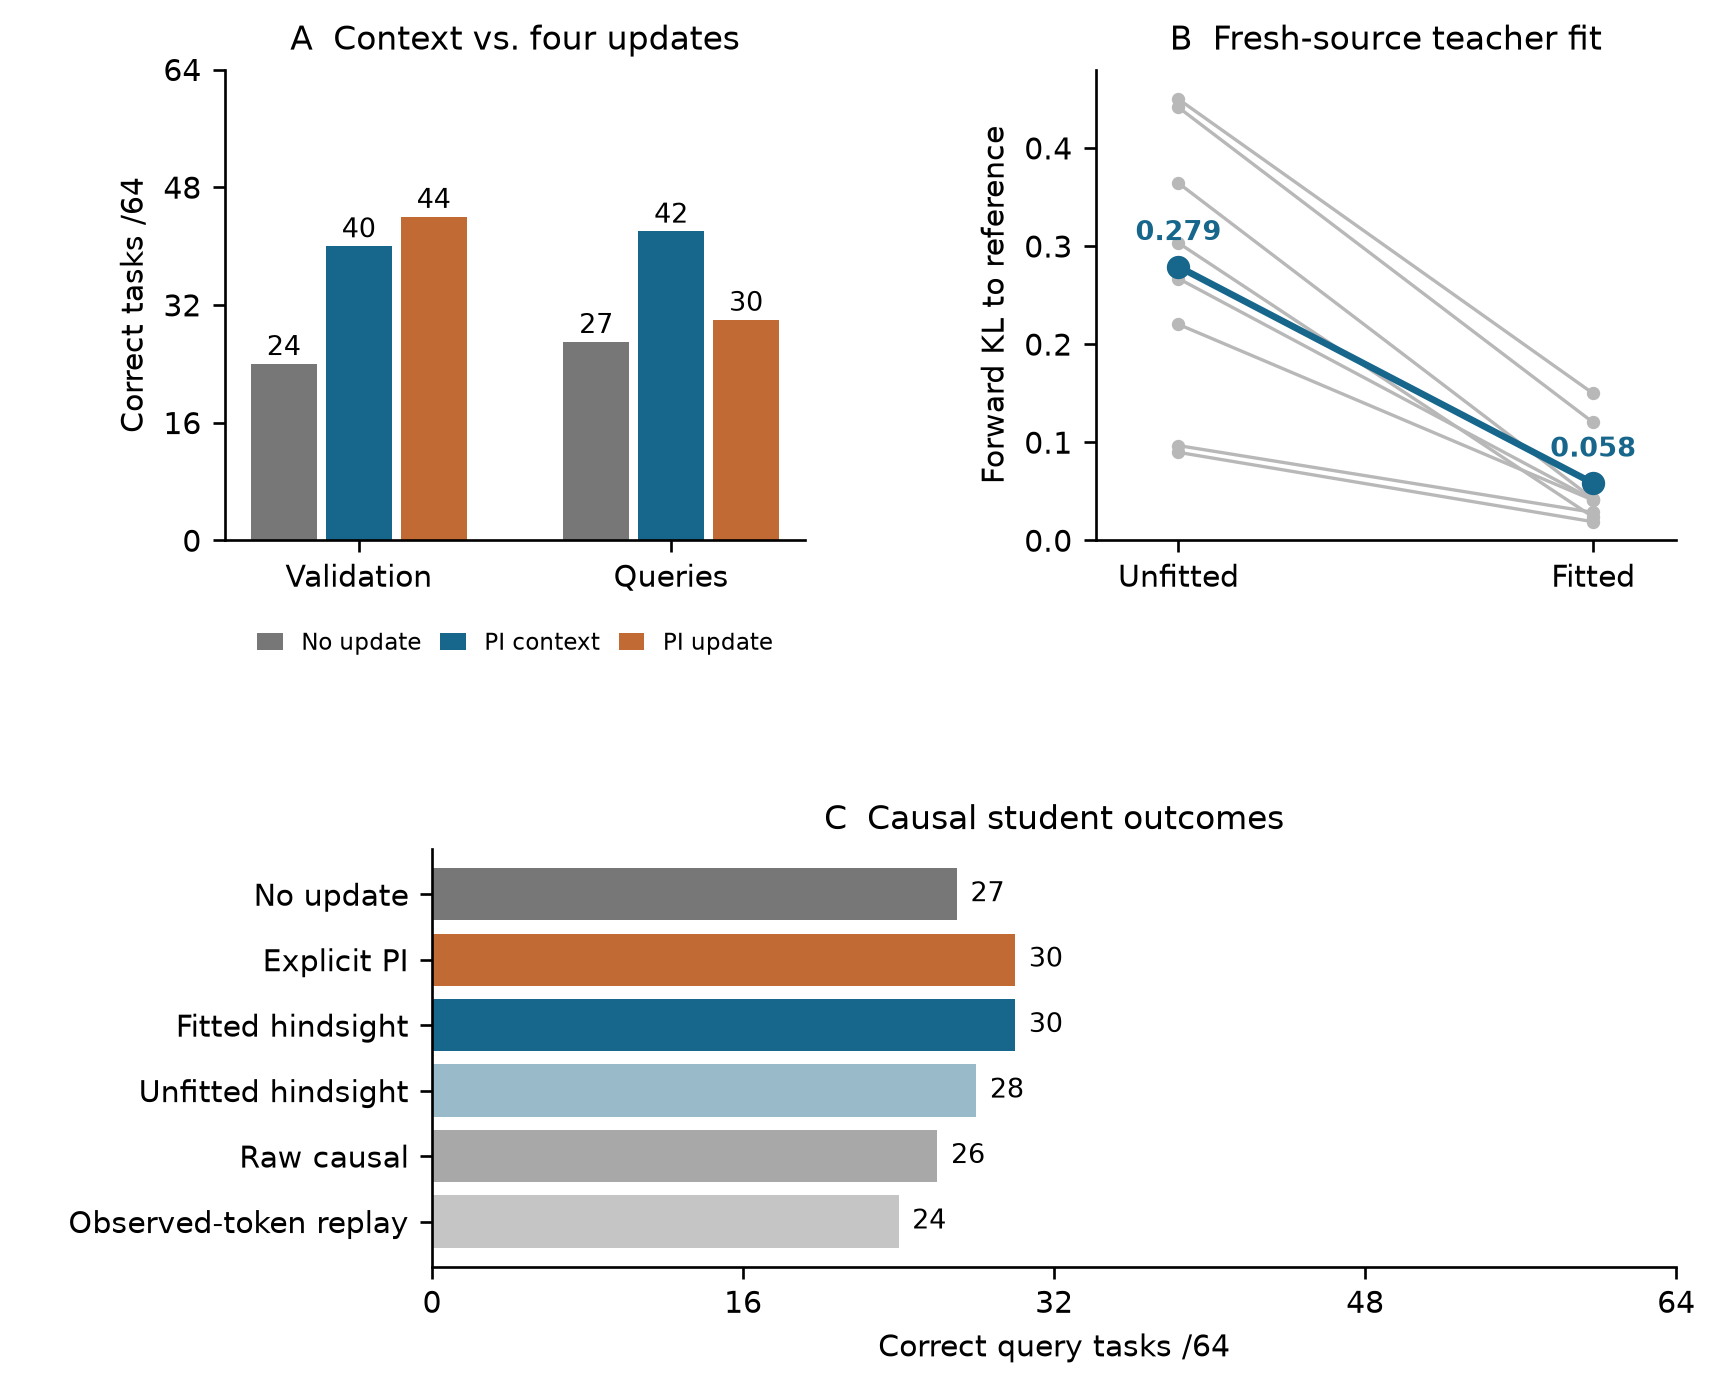
\includegraphics[width=\linewidth]{figures/context-fidelity-transfer.png}
\caption{Contextual utility, teacher fidelity and causal student behavior are separate measurements. A: matched validation/query counts. B: selected-reference KL on each fresh source (gray) and its mean (blue). C: query totals after the teacher/control conditions. Counts include failures; the main fitted-teacher gain intervals span zero.}
\label{fig:empirical}
\end{figure}

\section{What the distributions teach}
\label{sec:diagnostics}

Direct PI conditions a fresh generation for each new task. Source distillation instead scores one frozen historical answer. The distinction can matter even when the lesson is correct: later distributions remain conditioned on earlier historical tokens, and a finite adapter update can fit different positions unevenly.

\subsection{Localize imitation rather than trust the average}

A numerical diagnostic exactly reconstructs all eight historical explicit-PI student updates and saves full-vocabulary distributions before training, for the target, and after step four at all 576 native action positions. Independent CPU float64 calculations verify tensor hashes, source/lesson identities, action IDs and predecessor alignment. Recomputed per-position KL and total variation differ from recorded values by at most $1.4\times10^{-6}$. No new response or query score is generated.

Source-equal mean KL falls from 0.246606 to 0.023334, and total variation from 0.061767 to 0.023210. Every source improves, with KL reductions of 84.5--94.0\%. The reduction is concentrated, however: 102 rule-text positions account for 98.54\% of total initial KL and 92.63\% after updating. All 35 initial disagreements in the most likely next token occur in the rule sentence. None occurs at the 150 scalar array-value positions; teacher, initial student and updated student share the same argmax there.

These are loss contributions and predictions, not gradient norms or a claim about the location of internal reasoning. Equal argmaxes also do not imply identical distributions. They show that the observed imitation objective primarily distinguishes the models where the rule is verbalized rather than where the output values are chosen.

\begin{figure}[htbp]
\centering
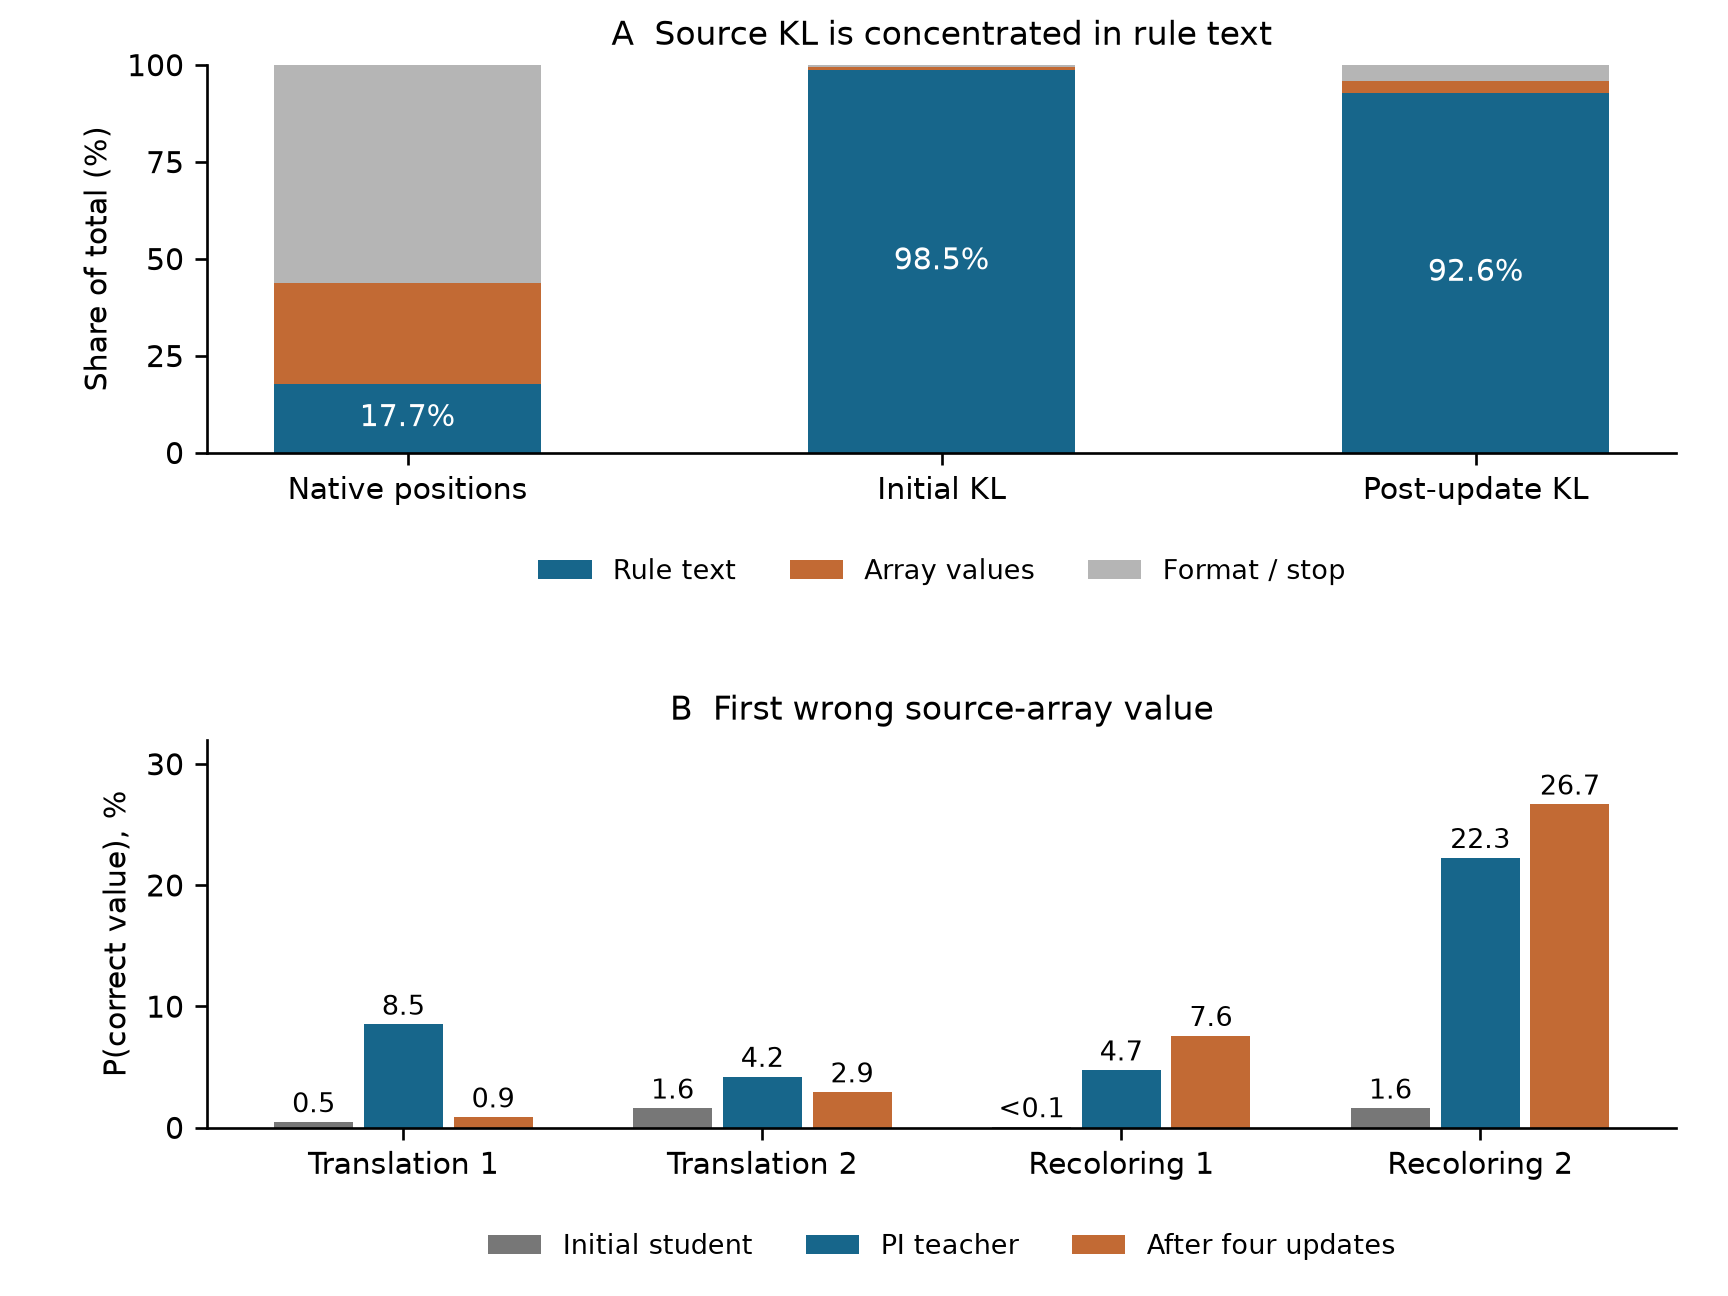
\includegraphics[width=\linewidth]{figures/source-fidelity-localization.png}
\caption{Aggregate imitation can obscure task-relevant corrections. A: pooled composition of native positions and summed KL. B: probability of the correct value at the first wrong array entry of each incorrect source. These are explicit-PI source-prefix targets, not fitted-hindsight predictions or fresh generations. All four target argmaxes remain wrong. Gold values are used only in the offline analysis.}
\label{fig:local}
\end{figure}
\FloatBarrier

\subsection{First-error targets remain weak or unevenly fitted}

At the first wrong array value of all four incorrect sources, the PI target still prefers a wrong value. For one translation source, the historical answer emits 8 where 0 is required. The PI teacher raises the correct value's probability from 0.46\% to 8.50\%, while the updated student reaches only 0.86\%, despite a 92.4\% reduction in source-average KL. At both recoloring first-error positions, the fitted student instead exceeds the teacher's correct-value probability.

Thus low average loss does not certify adequate retention of a localized corrective signal. Nor would perfect fitting make a target useful when it still strongly favors an erroneous source action. The analysis distinguishes weak targets, uneven finite fitting and transfer beyond historical prefixes; it does not identify one as the complete cause of the query gap.

An offline analyst's interpretation of the eight fixed lessons agrees with all 680 inspected generated input/output pairs. This verifies the supplied procedures on those examples, not model comprehension, uniqueness of the inferred rule or correctness on arbitrary inputs. Query answers used in this diagnosis never become proposer or update inputs.

\subsection{More explicit framing is not an established repair}

A separate scoring diagnostic adds an instruction that historical prefixes are fallible; another arm also exposes the complete original attempt and binary feedback. Neither receives source gold. Across the four first-error positions, mean correct-value probability is 0.09926 for original PI, 0.07758 with the fallibility instruction and 0.14346 with the richer context. The latter increase comes from one translation source; the other three worsen. Every first-error argmax remains the historical wrong token.

Across all 150 array values, averaged within each source and then equally across sources, the corresponding probabilities are 0.71821, 0.71570 and 0.71794. The first-error average is therefore not global improvement. The richer arm changes information as well as wording; these frozen-prefix scores neither establish a consistency-bias mechanism nor measure new-answer accuracy or student transfer.

\section{Learning the proposer with actual update reward}
\label{sec:proposer}

The black-box outer objective is implemented and was exercised in a subsequent development run. A throughput qualification first selects a repeat-stable batch-eight schedule by measured speed, not accuracy. Four of sixteen outputs differ from singleton decoding, so the next dose comparison uses new matched controls: no update 24/64 validation tasks, direct PI 40/64, four updates 42/64 and sixteen updates 44/64. Its predeclared rule selects sixteen only when better than four, preferring four on ties. Query outcomes do not enter this choice. The two-answer advantage is exploratory, not a confirmed transfer result.

The proposer-training run then uses 32 new meta-training sources, eight per family. Each group samples four PI candidates at temperature 0.7. Usable candidates induce matched sixteen-step student updates scored on four validation tasks. Leave-one-out REINFORCE uses post-update exact-match reward and sequence log-probabilities at the sampling temperature. A source-constant no-update baseline does not change within-group advantages.

Independent audit verifies all 32 groups, 128 proposals and 14 actual proposer optimizer updates. The remaining 18 groups have tied rewards and correctly perform no optimizer work. Of the proposals, 115 are usable and 13 are not; one hits the generation cap. Saved native tokens, regraded outcomes, checkpoint changes and Adam step counters were checked on CPU. Cached sampling and full teacher-forced token log-probabilities have a maximum absolute per-token discrepancy of 0.3050635 nats, a disclosed numerical limitation.

This establishes execution of real student-update reward training, not held-out teaching improvement. The reward reuses a small training-validation set, and no complete matched frozen-versus-trained fresh-source comparison is available. Training reward, optimizer activity and a runnable checkpoint are not substitutes for that comparison.

\section{Relation to existing methods}

On-policy self-distillation (OPSD) provides the aligned distribution interface: a teacher conditions on privileged solutions while the causal student learns on its own generated prefixes \citep{zhao2026selfdistilled}. Our question adds source-derived intervention selection by transferred update value and subsequent policy assignment from raw completed experience.

PAST already constructs a teacher with complete-trajectory privilege and distills onto unchanged student prefixes \citep{feng2026past}. Its analysis includes the possibility that a perfect privileged teacher does not help a causal student. Hindsight access or a teacher/student gap is not new in itself. The design here specifically targets post-update cross-task selection and amortization of the selected action distributions.

LOPD makes privileged context a learnable latent representation composed from retrieved successful experiences \citep{zhang2026latent}. This is a precedent for learnable supervision construction. Our proposer uses one source episode and a black-box learning-value reward; the eventual raw-hindsight scorer predicts policies without generating a context.

Meta Pseudo Labels directly optimizes a teacher through the performance of the student it trains, including a practical one-step approximation and hard-label REINFORCE \citep{pham2021metapseudolabels}. Valuing teaching by learning and avoiding a complete unrolled optimization graph therefore have clear precedents. Bidirectional teacher distributions for autoregressive generation also predate this work \citep{chen2020bertgeneration}.

Recent thinking-model self-distillation diagnostics report that contextual teacher advantages can fail to survive training, with evidence involving long-budget reasoning and deliberation markers \citep{kaur2026rethinking}. The short-array evidence here does not establish the same mechanism. It reinforces the methodological need to measure the resulting causal student.

The object of study is the combination: source-derived candidates, actual-update cross-task reward, no-update selection and direct raw-experience policy assignment. This report makes no exhaustive priority claim and reports no matched superiority comparison with these methods.

\section{Interpretation and next scientific question}

The central distinction is between \emph{information that helps inference} and \emph{supervision that causes useful learning}. A source-derived lesson can solve fresh tasks in context while supplying poor distributions on the old source prefixes. A teacher can generalize a distribution-matching objective while the target itself has limited learning value. A close neutral prediction can still cause a harmful update.

These observations motivate the actual-update outer reward, but do not prove that candidate search or proposer training will resolve the bottleneck. Repeated validation can overfit, especially with few tasks and tied rewards. The main component comparison has eight learning clusters, familiar families and one principal execution seed. The adapted distribution, adapter capacity and finite optimization recipe all affect interpretation.

The next decisive question is whether a strong, fixed source-only proposer supplies a teaching signal that reliably improves the causal student on different tasks. Only then is there a clear target for testing whether the learned hindsight teacher preserves that value. This ordering avoids optimizing distribution fidelity around weak supervision. Competition mathematics is a prospective setting for that question, not an experiment reported here.

The scalable destination remains attractive: spend outer-loop compute discovering how to teach, then perform ordinary updates through direct scoring of completed experience. The implemented method makes this direction executable, and the component study shows where evidence is still required. Useful context, accurate policy assignment and useful learning must be measured separately.

\appendix
\section{Historical comparisons and evidence boundaries}
\label{app:evidence}

\subsection{Earlier development remains part of the record}

The first complete development protocol uses Qwen3-4B-Instruct-2507 with three PI candidates on sixteen source episodes across eight familiar families. It reports no intervention at 49/128 queries, validation-selected direct PI at 48/128 and selected adaptation at 47/128. It completes 1,728 planned evaluation records and 192 student steps. Generic advice and mismatched-source PI are direct-context controls in that protocol, not matched parameter-update controls. Later Qwen3.5 development changes do not erase this negative result.

The balanced Qwen3.5 study subsequently reports validation 24/64 to 44/64 and queries 23/64 to 36/64 after source updates, while direct PI scores 48/64 and 43/64 respectively. The fresh fitted-teacher study instead reports validation 24/64 to 44/64 and queries 27/64 to 30/64. Identical validation totals do not make these the same tasks or a controlled rerun; source episodes, lessons and evaluation inputs change.

For the fresh study, query family totals for baseline/direct PI/explicit-PI update are translation 0/7/4, denoising 4/10/4, recoloring 8/10/7 and gravity 15/15/15, each out of sixteen. The fitted-hindsight teacher has different family outcomes despite sharing the explicit-PI aggregate.

\subsection{Order and state controls}

Two students with large validation/query differences are reconstructed from the prescribed updates. Identical prompts are replayed in original, reversed and interleaved order. Current token outputs agree exactly across all layouts and reproduce historical text, grades, lengths and cap status. Recorded parameters, buffers and optimizer hashes remain unchanged. Historical generation token IDs were not saved, so historical token equality is not asserted. This checks the suspected order effect for the two selected students, not universal numerical invariance.

The later batch qualification differs from singleton generation on four of sixteen outputs. Repeat stability within a schedule does not establish equivalence across schedules; subsequent batch-eight controls are kept separate.

\subsection{Paired interpretation and missing confirmation}

The main fitted-teacher comparison is development evidence. Source-cluster intervals account for dependence among the queries sharing one update, but not every uncertainty from task generation, model choice or iterative research. The fixed external proposer and instruction-enforced source restriction further bound the claim.

The last recovered expanded proposer-evaluation receipt records nine of sixteen source episodes complete. Its backup is a non-atomic snapshot, not a terminal proof of the remote run. No completed shared-weight learning result is recovered. Neither partial study contributes a completed aggregate in this report; missing outcomes are not inferred. A planned fitted-causal control also changes serialization relative to the future-aware mode, so it would not be a pure attention-mask ablation without further design work.

\section{Source-level diagnostic details}

The independently audited source-fidelity reconstruction covers 576 original action positions: 102 verbal rule positions, 150 scalar array values, and the remaining formatting/stopping positions. All 35 initial teacher/student top-choice differences are in rule text; 30 resolve after updating and five new ones appear. None occurs among array values. These are correlated positions in eight sources, not independent token-level experimental replicates.

At the four first erroneous array values, the historical wrong value remains the PI target's argmax. The first translation source's correct probability changes from 0.0046 initially to a target of 0.0850 and an updated value of 0.0086. The other translation and two recoloring examples are preserved in the released derived record. Source gold is used only for this offline localization, after target distributions have been scored.

The framing audit checks all 576 positions and 150 scalar values, with recomputation differences within $10^{-6}$. Every first-error argmax remains wrong. Richer context raises one correct-value probability from 0.04206 to 0.43704 and lowers the other three; the four-position mean does not measure array-wide correctness or learning.

\section{Computational footprint and reproducibility}

The main experiments ran on an NVIDIA H100 80 GB. Full-vocabulary targets require substantial storage as well as scoring memory; the implementation does not replace them with a sparse approximation. Separate teacher/student adapters limit parameter-update storage, but do not remove backbone activation or vocabulary costs.

\begin{table}[htbp]
\centering\scriptsize
\caption{Completed invocation work, not total project expenditure or an efficiency benchmark. Proposer likelihood forwards/backwards are noted separately.}
\label{tab:work}
\begin{tabular}{L{1.72in}rrrrr}
\toprule
Invocation & Generated & Source scores & Student steps & Teacher steps & Elapsed\\
\midrule
Balanced transfer (021) & 384 & 8 & 32 & 0 & 24m54s\\
Fitted-teacher study (023) & 512 & 61 & 160 & 64 & 46m42s\\
Direct PI/order (024) & 224 & 2 & 8 & 0 & 16m53s\\
Source fidelity (025) & 0 & 16 & 32 & 0 & 1m26s\\
Batch qualification (026) & 80 & 0 & 0 & 0 & 1m32s\\
Validation dose (027) & 256 & 16 & 160 & 0 & 4m43s\\
Proposer training (028) & 748 & 115 & 1,840 & 0 & 43m04s\\
Prefix framing (029) & 0 & 16 & 0 & 0 & 28s\\
\bottomrule
\end{tabular}
\end{table}

The fitted-teacher invocation also records two discarded qualification teacher steps/exposures, making 66 steps and 258 exposures including qualification; the table separates its main 64-step fitting recipe. Fresh source preparation adds eight generations and eight external proposer sessions. Proposer training's 748 generated sequences include all 128 proposal draws; its fourteen optimizer updates also require 56 likelihood forwards and 56 backward sequences, separate from the 115 teacher/source scores. Reused baseline records are not new generations. These counts describe completed components, not a complete campaign invoice or a matched total-cost comparison.

The public repository separates three reproduction levels: offline verification of released evidence; deterministic generation and CPU checks of the learning machinery; and new model execution requiring the declared model, GPU, storage and configuration. A passed CPU test does not replicate a GPU learning effect. Rebuilding figures from historical records does not generate fresh scientific observations.

The canonical report source, figure assets and bibliography accompany the PDF. Result identities, configuration hashes, paired observations, derived counts and audit receipts identify the numerical claims. Raw full-vocabulary tensors and model checkpoints are distinguished from compact distributable analysis records; their availability is not implied by a figure-rebuilding command. The original private research archive is preserved rather than rewritten into a public history.

\bibliographystyle{plainnat}
\bibliography{references}
\end{document}
